\section{Evaluating the Classifier Performance}

The performance of a classifier is not solely determined by its ability to make correct predictions. There are several
measures of performance, each emphasizing a different aspect of the classifier's behavior. Choosing the right measure of
performance is vital as it directly impacts the optimization procedure during training and influences how well the model
generalizes to unseen data. Therefore, it is important to understand these measures in detail.

\subsection{Loss Function: The Objective of Training}

The loss function quantifies the discrepancy between the model's predictions and the actual targets in the training set.
It provides an objective measure that we strive to minimize during the training process. Cross-entropy loss, also known
as log loss, is a commonly used loss function for classification tasks, including ours:

\begin{equation}
    L(\mathbf{y}, \mathbf{\hat{y}}) = -\frac{1}{N}\sum_{i=1}^{N}\sum_{j=1}^{M} y_{ij} \log(\hat{y}_{ij})
\end{equation}

where $N$ is the number of samples, $M$ is the number of classes, $\mathbf{y}$ is the true label, and $\mathbf{\hat{y}}$
is the predicted label.

\subsection{Validation and Test Sets: Generalization Checkpoints}

\begin{figure}[htbp]
    \centering
    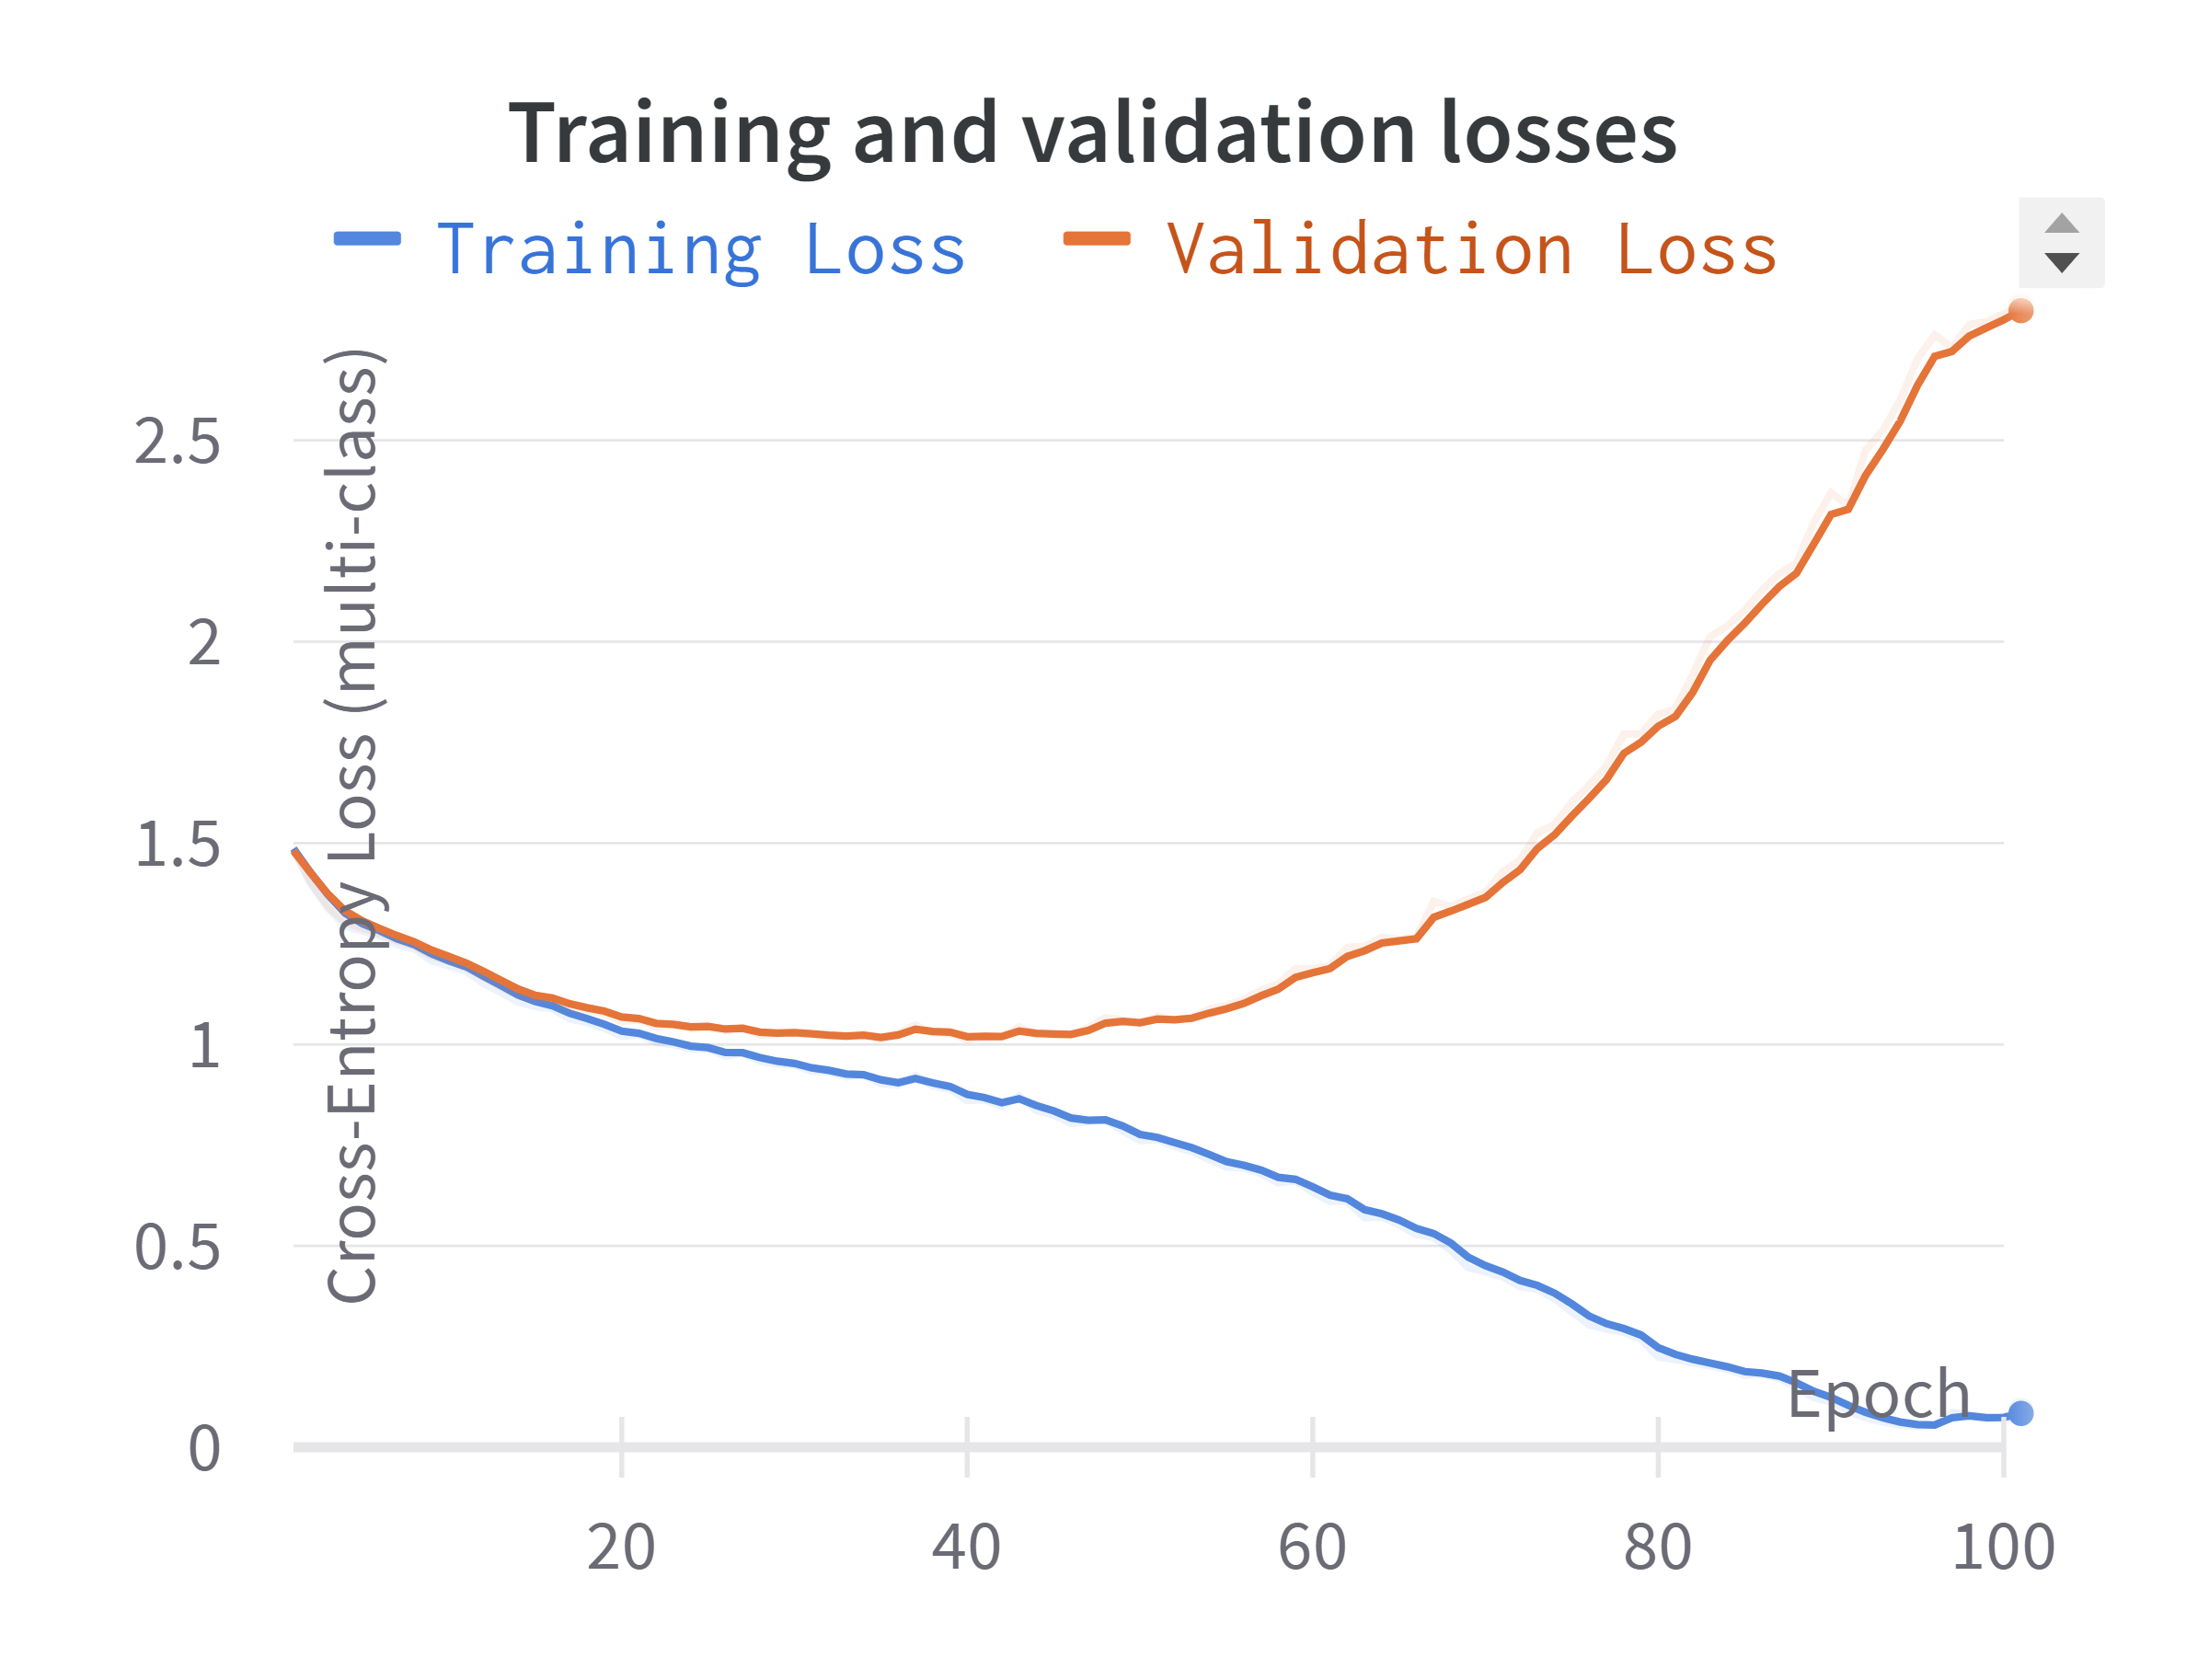
\includegraphics[width=0.8\textwidth]{figures/plots/ml/losses.png}
    \caption{Training and validation losses during the training process. \gls{ftt} with 2 blocks and embedding size
        of 256 was used on the plot (see \autoref{sec:ftt}). Around the 30th epoch, the training loss starts to
        decrease while the validation loss starts to increase, indicating that the model is overfitting to
        the training data. It is at this point that the checkpoint is saved and used for evaluation.}
    \label{fig:losses}
\end{figure}

To assess the generalization ability of the classifier, the dataset is typically divided into three subsets: training,
validation, and test sets. The training set is used to adjust the model's parameters, the validation set is used to tune
the hyperparameters and provide an unbiased evaluation of the model during training, and the test set is used to assess
the performance of the fully-trained model.

During training, not only is the training loss monitored, but also the validation loss. The validation loss provides an
unbiased estimate of the model's performance on unseen data and is crucial for preventing overfitting. If the training
loss continues to decrease while the validation loss starts to increase, the model is likely overfitting to the training
data and failing to generalize to unseen data (see \autoref{fig:losses}). The point at which the validation loss is
minimized is typically chosen as the stopping point for training (early stopping).

\subsubsection{Performance Metrics: More than Accuracy}

While the loss function provides a measure of the classifier's performance, it does not tell the whole story. For
instance, the loss function does not capture the trade-off between correctly identifying positive instances
(sensitivity) and correctly identifying negative instances (specificity). To address this, several other performance
metrics are commonly used to evaluate classifiers.

\subsubsection{Confusion Matrix: A Comprehensive Performance Snapshot}

The confusion matrix provides a comprehensive view of the classifier's performance. For a binary classification task, it
is a 2x2 matrix where the rows correspond to the true classes and the columns correspond to the predicted classes:

\begin{equation}
    \begin{pmatrix}
        \text{TP} & \text{FP} \\
        \text{FN} & \text{TN} \\
    \end{pmatrix}
\end{equation}

where TP (true positive) is the number of positive instances correctly identified as positive, TN (true negative) is the
number of negative instances correctly identified as negative, FP (false positive) is the number of negative instances
incorrectly identified as positive (Type I error), and FN (false negative) is the number of positive instances
incorrectly identified as negative (Type II error).

In our context, the confusion matrix can be extended to a multi-class scenario, leading to an MxM matrix for an M-class
classification task. Moreover, to reflect the underlying data distribution, the confusion matrix should be weighted,
with each instance contributing to the confusion matrix proportional to its weight.

The confusion matrix serves as the basis for several other performance metrics, including accuracy, F1 score, and area
under the ROC curve (AUC-ROC).

\subsubsection{Weighted Confusion Matrix: Accounting for the Data Distribution}

When using machine learning in high-energy physics, the data distribution used to train the model often differs from the
real-world data distribution we aim to make predictions on. This is due to the Monte Carlo simulations we use to produce
our training data. While these simulations are designed to model the physical processes as accurately as possible, they
do not perfectly represent the real data distribution.

This discrepancy is resolved by attaching a weight to each event in the simulation. The weight represents the ratio of
the number of expected events in the real data to the number of events in the simulated data. Using these weights, we
can then scale the distribution of the simulated data to match the expected distribution of the real data.

When evaluating the classifier's performance, it is crucial to use a weighted confusion matrix to account for these
event weights. In the weighted confusion matrix, each instance contributes to the matrix proportional to its weight. The
weighted confusion matrix for a binary classification task is given by:

\begin{equation}
    \begin{pmatrix}
        \text{TP}_{w} & \text{FP}_{w} \\
        \text{FN}_{w} & \text{TN}_{w} \\
    \end{pmatrix}
\end{equation}

where each term (TP, FP, FN, TN) is the sum of the weights of the corresponding instances.

The performance metrics derived from this weighted confusion matrix (accuracy, F1 score, AUC-ROC, etc.) then reflect the
performance of the classifier on the actual data distribution we are interested in. Hence, using a weighted confusion
matrix enables us to evaluate and optimize our classifier in a manner that is directly relevant to our ultimate goal:
the accurate classification of ttH events in the actual LHC data.

\subsubsection{Accuracy: The Proportion of Correct Predictions}

Accuracy is the most intuitive performance metric. It is the proportion of total predictions that are correct and can be
calculated directly from the confusion matrix:

\begin{equation}
    \text{Accuracy} = \frac{TP + TN}{TP + FP + FN + TN}
\end{equation}

\subsubsection{F1 Score: The Balance Between Precision and Recall}

The F1 score is the harmonic mean of precision and recall, providing a balance between the two. Precision (also known as
positive predictive value) is the proportion of positive identifications that were actually correct, while recall (also
known as sensitivity) is the proportion of actual positives that were identified correctly. The F1 score can be
calculated as:

\begin{equation}
    \text{F1 Score} = 2 \cdot \frac{\text{Precision} \cdot \text{Recall}}{\text{Precision} + \text{Recall}}
\end{equation}

\subsubsection{ROC Curve and AUC: The Trade-off Between Sensitivity and Specificity}

The receiver operating characteristic (ROC) curve is a plot of the true positive rate (recall or sensitivity) against
the false positive rate (1 - specificity) for different classification thresholds. The area under the ROC curve
(AUC-ROC) measures the classifier's ability to distinguish between classes. A perfect classifier has an AUC-ROC of 1,
while a random classifier has an AUC-ROC of 0.5.

These metrics, combined with the loss function, provide a comprehensive view of the classifier's performance and guide
the optimization process during training. They also provide a robust measure for comparing different classifiers or the
same classifier with different hyperparameters.